\cleardoublepage
\singlespacing
\chapter{BACKGROUND}
\label{c:background}
\doublespacing\nointerlineskip

\section{Internet-of-Things}

Internet-of-Things is a powerful paradigm in the scenario of modern wireless
telecommunications. It refers to the pervasive presence of uniquely identifiable
objects (things) around us - such as Radio Frequency IDentification (RFID) tags,
sensors, actuators, mobile phones, etc, which would be able to interact with
each other forming a network like structure.~\cite{Atzori20102787}

\section{Machine-to-Machine}

Machine-to-Machine refers to technology that enables both wireless and wired
systems to communicate with other devices with the same ability. Thus a device
(equipped with sensors) could capture an event (such as photodetector,
    temperature, etc), which is relayed through a network (wired, wireless or
      hybrid) to an application which will translate that into a meaningful
    information to perform action upon (e.g. turn on actuators).

\subsection{Wireless Sensor Networks}

Wireless sensor networks are a network of sensor nodes.
Sensor nodes are equipped with low-power, low-cost, and failure-prone
sensors or actuators. Sensor networks are networks of sensor nodes that connect to the physical space that are intrumented to produce data that could be meaningful
for further research. They collaborate to collect, process and disseminate
environmental information\cite{ArchanaBharathidasan}.

Sensor network could be homogeneous, meaning all nodes are identical with same
sensors, actuators and hardware setup. Sensor networks could also be
heterogeneous where nodes have different sensors, actuators and hardware setup.
Heterogeneous networks require higher level management and organization
resources. Wireless sensor networks are nodes that communicate through air by
sending electronic signals. Wireless communications aren't stable, as it is
highly influenced by environmental factors.

\section{Redundancy architecture}

%A distributed system usually consists of hosts that host services that clients or
%other services could read or write with some associated communication
%frequencies according to the application requirements. The
%problem of partial failures makes service redundancy a fundamental technique to
%distributed systems as it improves availability, eliminiates single points of
%failure. A system that is hardwired to get data from node X will fail when
%X fails. The problem of designing a system with replicas where node Y, which
%can provide the same service as X, can take over when X fails. To design such
%system, it is important to have a clear definition of a service such that it
%could be replicated onto heterogeneous hosts. It is
%also essential that the system could track and manage available replicas in the
%network. Autonomy is an important attribute of distributed systems since most
%of them would be left unattended for a long period of time; systems should be
%able to reconfigure and recover themselves in the event of failure.

Sensor networks are usually deployed in large scale and unattended in long
period of time. Sensor networks communicate with
low-power wireless radios to aid scientists in collecting spatial data that
could lead to more understanding of the environment. However, several
challenges such as node failures, message loss, and sensor calibration leaves
the effectiveness of sensor networks in question. With the assumption of spare
homogeneous resources, redundancy is used in sensor networks to increase fault
tolerance against node failures. The system is designed with backup nodes that
could automatically recover and replace should one node fail.

\begin{comment}
\section{Component Based Middleware}

Middleware enables communication and management of data that simplfies 
complex distributed applications.

As most applications for wireless sensor network involves management of data and
communication between network of nodes, middleware is integral in providing
a unified experience for implementing more complex architecture such as 
service-oriented architecture.

However, the separation of design abstractions between low-level hardware and
high-level application logic has not been successful in sensor based systems.

It is also not successful in terms of making them adapatable and evolvable 
for new services in new environments.

Next section presents an instance of a component based middleware.

\subsection{WuKong: Intelligent Middleware for Flexible Sensor Configurations in
  M2M Systems}

WuKong: Intelligent Middleware for Flexible Sensor Configurations in M2M
Systems~\cite{Reijers} consists of frameworks that supports flexible
configurations of application specifications from flow-based programming.
It uses component based architecture where services could be represented by
software components which will be deployed to a set of hosts, and each host
could hold more than one component.
\end{comment}

\section{WuKong: The intelligent middleware for M2M applications}

\subsection{Goal}

Deployment and development for M2M applications are in its infancy today. As
many applications are still single purpose in homogeneous networks with
specific network protocols. The hardware has a fixed range of sensors, and the
applications cannot be easily ported to other platforms.

The existing middleware support that decouple high-level application design
abstractions and low-level hardware has not been successful.

In Intel-NTU Center Special Interests Group for Context Analysis and Management 
(SIGCAM), we have been collaborating on a project, called WuKong, aiming to develop 
an intelligent middleware for developing, and deploying machine-to-mahicne 
(M2M) applications with ease. The main contribution of this project is to support
inlligent mapping from a high-level flow based program (FBP) to
self-identified, context-specific sensors in a target
environment\cite{Reijers}.

\subsection{Flow Based Programming}

\begin{figure}[h!]
\caption{A FBP application}
\centering
    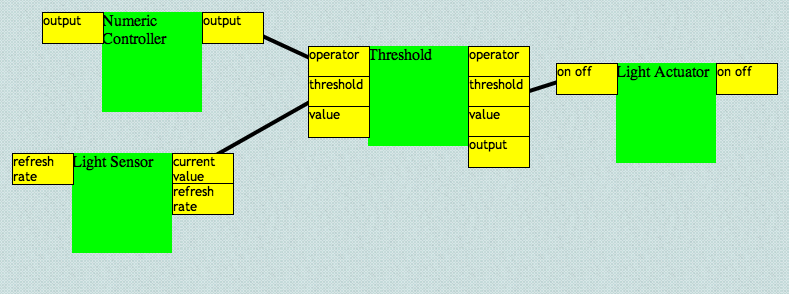
\includegraphics[width=\linewidth]{figures/fbp-application}
\label{fig:fbp-application}
\end{figure}

M2M applications are by definition distributed where the application
requirements involve a network of nodes collaborating for some common 
goals. M2M applications are typically defined by its flow of information
between components, as opposed to more traditional applications that focus more
on local information processing.

Flow Base Programming is best suited for describing M2M applications as it
allows the developers for the applications to focus more on the
abstraction meaning of the components instead letting the unimportant details
such as the hardware to stick right in the face. The result application will
contain all necessary information for the framework to construct low-level
details to implement the flow.

Applications are designed and constructed on FBP canvas by dragging a set of
abstract components from the library as illustrated in Figure~\ref{fig:fbp-application} 
Each component is
illustrated by a green block, each block has a set of properties, each with
different access modes, such as readonly, writeonly, readwrite. Properties on
the left of the greenblocks are properties that could be written, and
properties on the right are readable. Components are connected by links, which
is drawn by linking two properties in different components.

Some components represent physical hardware such as a sensor, or an actuator
while some other components could represent virtual processes such as
mathmatical computations, comparisons, etc. However, the final physical implementations
of the components are only made during application deployment by the Master but
not during FBP construction.

Components expose their interface through properties. A link is only made with
properties with matchinkg data type. The FBP applciation in
Figure~\ref{fig:fbp-application} illustrates a simple scenario where the light actuator
will turn on the light if light level drops below some value. The Numeric
Controller component will be assigned to a user input device used by users to
set its desire light threshold, which its output is sent to Threshold
component. The light value is sensed from Light Sensor component and sent to
Threshold. If the light value sensed is below the threshold value, Threshold
will output a boolean to set the on off property of Light Actuator to turn the
device, which will be deteremined during deployment, that it is represented by
on or off.

\subsection{Sensor Profile Framework}

While FBP defines the logical view of an application, WuKong profile framework allows
tracking, identification of physical resources within the Sensor Network.
There are a range of sensors which provide similar functionality with different
level of quality, it could model the sensor capability to enable handling
heterogeneous sensors and provide a common abstraction for the logical view.

There are two main concepts in Sensor Profile Framework, WuClasses and
WuObjects. WuClasss model components by exposing a number of properties
describing, and allow access to, a specific resource represented by the class.
Drawing from the example in Figure~\ref{fig:fbp-application}, the on off property of Light
Actuator component is boolean writeonly. WuClass also implements an update
function to describe a component's behavior. For
example, Threshold has four properties: operator, threshold, value, output. The
output value is determined from the previous 3 properties that it returns true
when the value is lower or higher than the threshold which depends on the value
of the operator, and it returns false otherwise.


WuObjects are the main unit of processing that are hosted on the nodes. Each
WuObject is an instance of WuClasses. It allows the framework to achieve
4 responsibilities:
\begin{enumerate}
\item Allow the Master to discover the current status of a node with the list
of WuClasses and WuObjects it has.
\item Create new WuObject instances on a node to start receiving data and doing
local data processing.
\item Trigger executions in WuObjects, either periodically or as a result of
changing inputs.
\item Propagate changes of properties between linked properties in different
components, which may be hosted locally or remotely.
\end{enumerate}

\subsubsection{Property Propagation}

The profile framework is in charge of communication between WuObjects as
well, which are not necessarily on the same nodes. Profile Framework monitors
the changes in properties and propagate the changes to the connected WuObjects.
For example, if a Temperature WuObject is connected to a Threshold WuObject,
the changes in Temperature current value property will trigger propagation from
the Profile Framework to propagate the new value in current value to the
Threshold WuObject connected property, and since Threshold WuObject could be on
a different node, the framework will take care of this by initiating
a wireless connection between the nodes to send the data over. Once a new value
has been set, Threshold WuObject will also trigger its update() function to
recompute its output properties which in turn would cause another chain of
propagation to the linked WuObjects.

\subsection{Compilation and Mapping}

\begin{figure}[h!]
\caption{WuKong application build flow}
\centering
    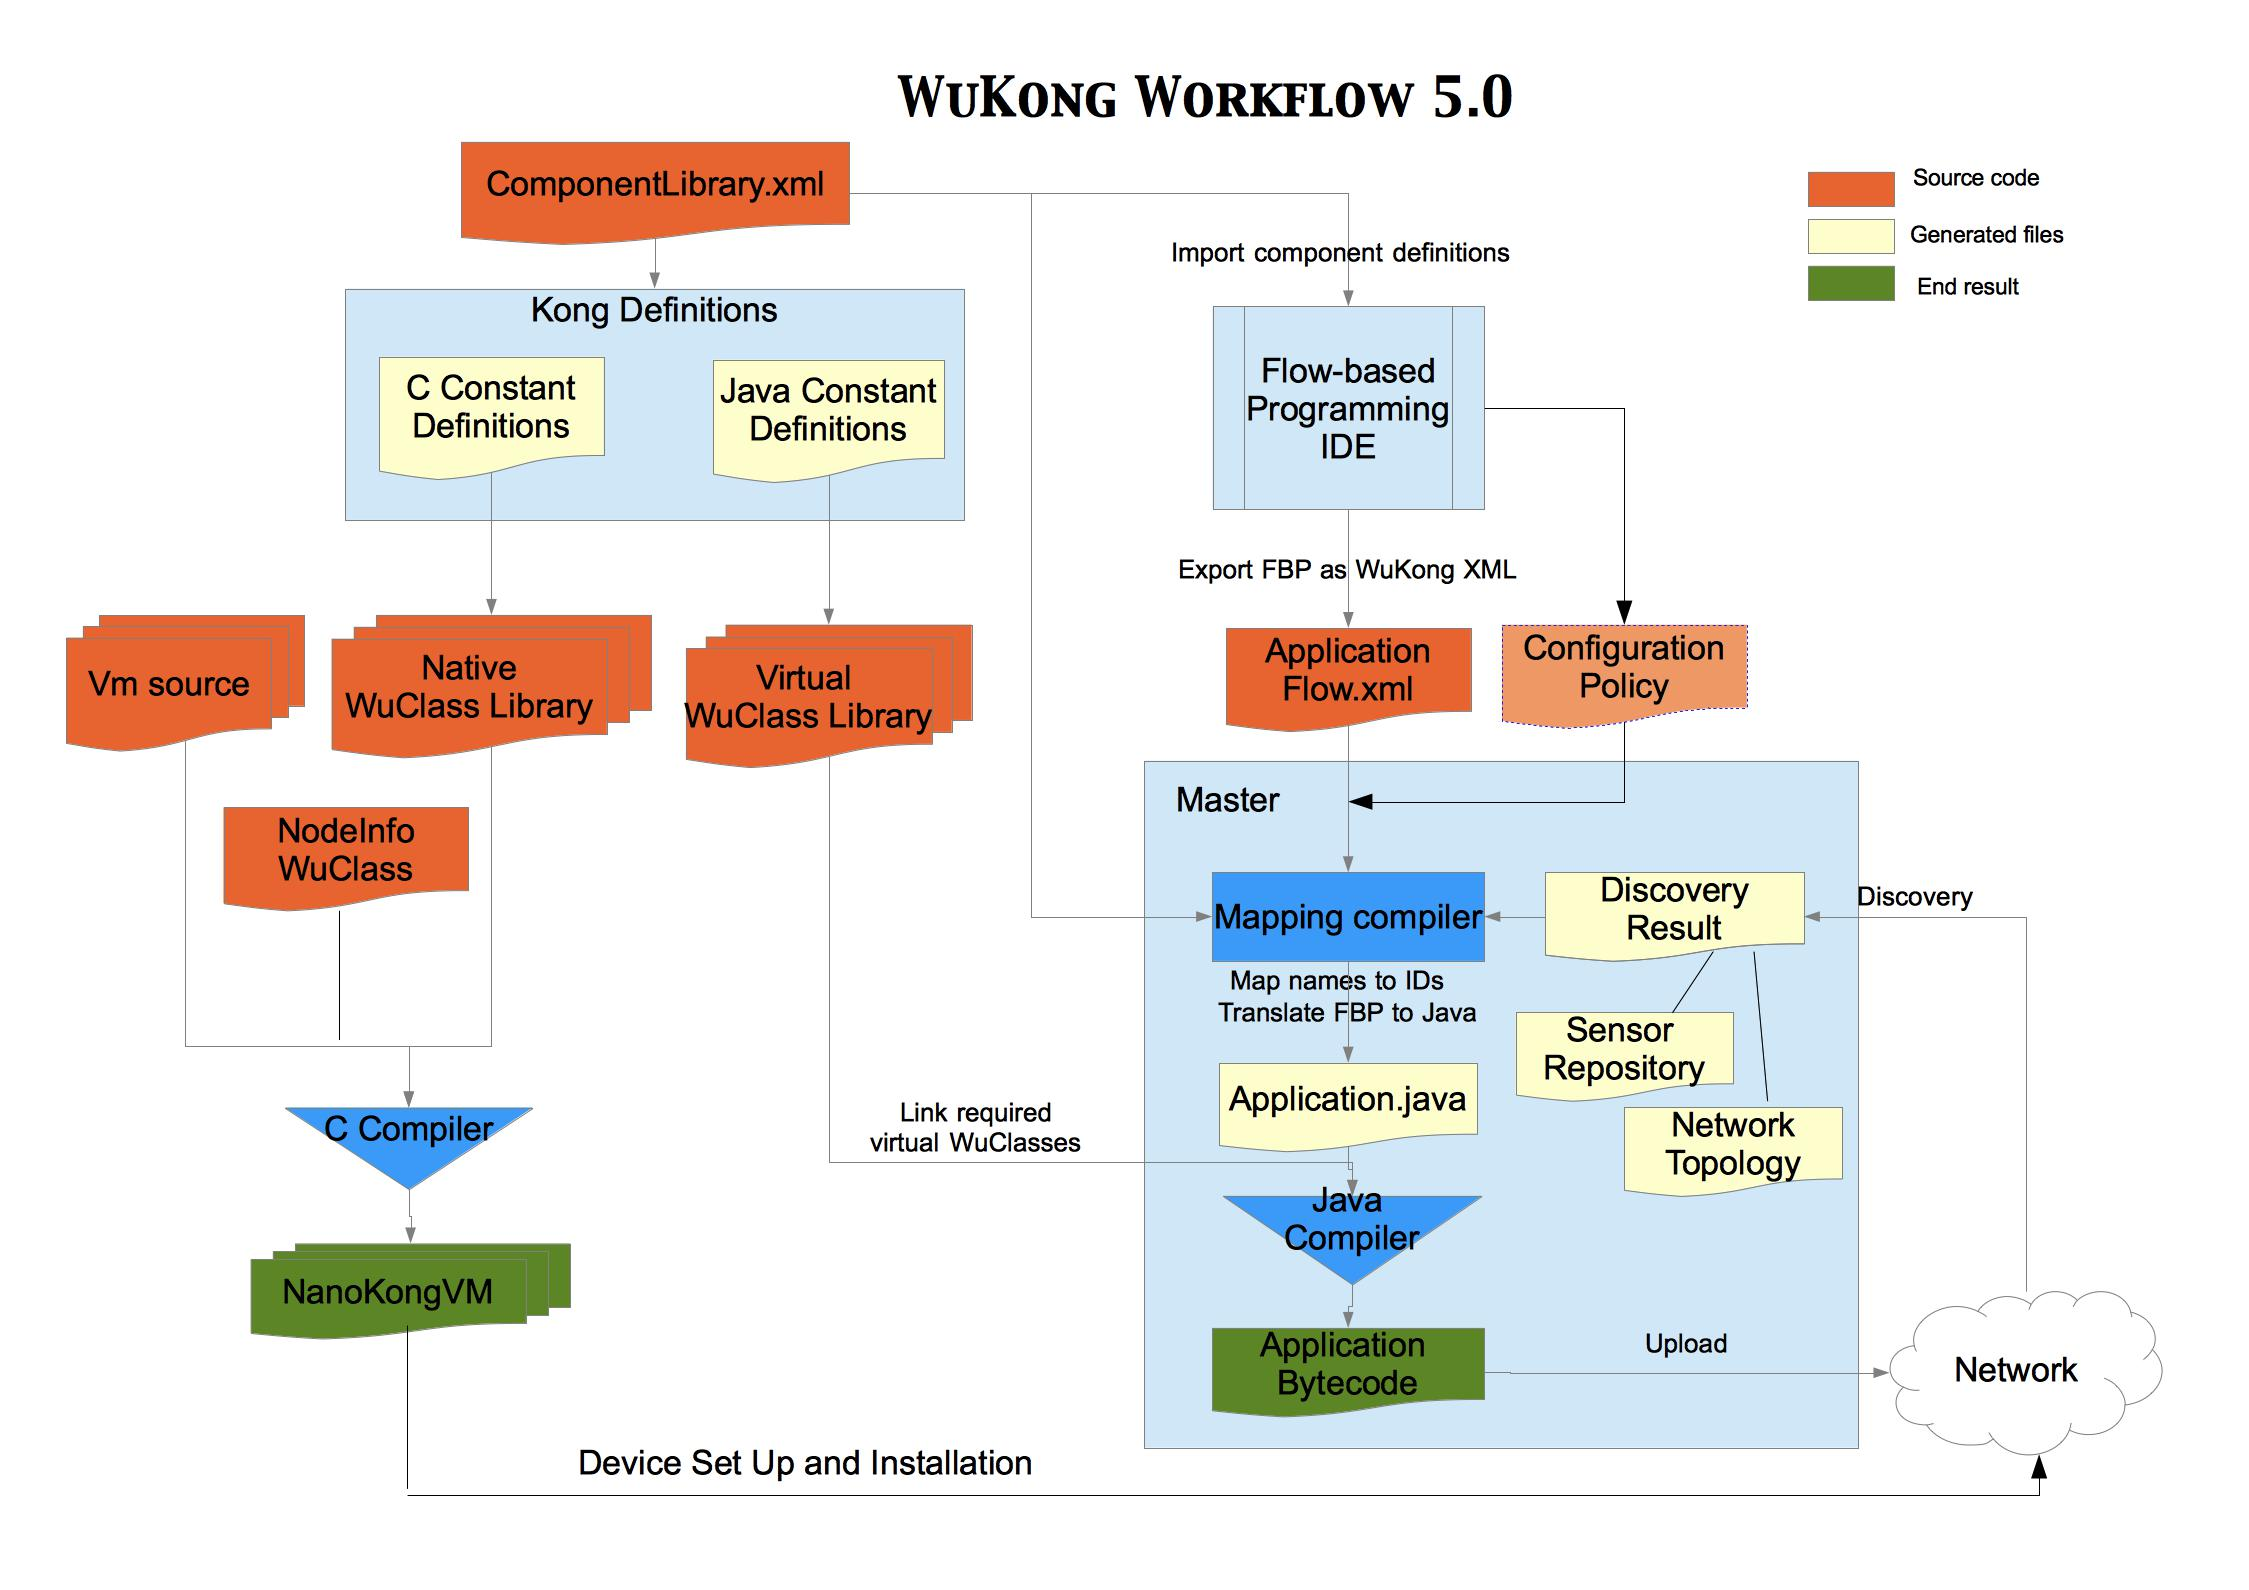
\includegraphics[width=\linewidth]{figures/wukong-flow}
\label{fig:wukong-flow}
\end{figure}

Figure~\ref{fig:wukong-flow} shows the overview of WuKong's build flow. The
left part represents the build process for NanoKong VM which will be installed
on the sensor nodes as part of the WuKong framework. The top part represents
the build process for generating component libraries and Virtual WuClass
library which will be used in other parts of the process. The right part
illustrates the build process for FBP applications from being drawn in the IDE
to Java bytecode that will be transmitted to the nodes.

The FBP program from the IDE will be exported as XML to the Master, the Master
will then take this XML and passed to Mapper to generate a Java program that
will be executed on the nodes. Finally, the compiled code is then wirelessly
uploaded to the nodes in the network.

The Java code consists of many parts from different phases of the mapping process.
First, the Java code contains information about links between components that
were taken from the FBP XML passed in earlier from the IDE. A link contains the
source component id, destination component id. The library code for components
corresponding to the component ids are stored in the node if it is written in
native language, or uploaded as part of the Java bytecode if it is written in
Java language. Second, it contains information about the mapping from
application component ids to actual node identifications and positions. The
purpose of a mapping which separates from the actual link makes it easier to
substitude the actual host of the WuObject later during
reconfiguration from the Master. This mapping is created by the Master during
discovery phase that probe the network for node's capabilities in terms of
available WuClasses, then mapper will decide the final candidates that will be
hosting for a component. If no native version of a component is found on the
nodes, mapper will substitute with a Java version of it.

\subsection{System Progression Framework}

There are a few popular wireless communication protocols in M2M applications:
ZigBee, ZWave. It is expected that in the future more diverse
wireless nodes equipped with radios that support protocols such as low-power
bluebooth and WiFi that all have one or more powerful gateway to connect to the
outside world. In WuKong system, one of the gateways will take on the role of
higher management decision maker called \emph{Master} to making the decisions for
deployment and producing the configuration of wireless sensor networks.

